\chapter{Vergleich der Implementierungen}
\label{ch:vergleich}
Bisher wurden die Implementierungen nur in einem stationären Szenario mit dem Access Point in Reichweite getestet. 
Dies spiegelt jedoch nicht das Szenario der Arbeit im Tunnel wieder, bei der sich die Mitarbeiter sich regelmäßig bewegen und auch in Bereichen arbeiten, in denen kein AP WLAN zur Verfügung stellt. \\
Ein Test mit den Mitarbeitern war leider nicht möglich, da der Versuchsaufbau mit Powerbank, USB-Power-Meter und ESP8266 Feather zu ausladend und wegen der Steckverbindungen zu fragil für den Arbeitsalltag ist.
Auch das Mitführen des Versuchaufbaus durch den Autor ist nicht praktikabel, da die Versuche über mehrere Stunden durchgeführt werden müssen und in den Arbeitsbereichen auf der Tunnelbohrmaschine nur wenig Platz vorhanden ist, so dass die normale Arbeit behindert werden würde.
Dies ist insbesondere der Fall, wenn realistische Bewegungsprofile nachvollzogen werden sollen. 
Dazu müsste ständig ein Arbeiter verfolgt werden, das behindert diesen natürlich und ist auch nicht einfach möglich, da Gefahrenbereiche vom Autor mangels Sicherheitseinweisungen nicht betreten werden dürften.
Die Bedingungen wurden deshalb stationär simuliert.

\section{Simulationsumgebung}
Für ein realistischen Verbrauch mangelte es der bisherigen stationären Versuchumgebung an Reassiziationen (Wechsel des AP) und dem nicht vorhanden sein eines APs.
Dies soll durch abschalten des APs simuliert werden. \\
Es wurde ein Schema gewählt, in dem der AP nach jeweils 15 Minuten für fünf Minuten abgeschaltet wird. 
Für einen echten Arbeiter sind die Zeitabschnitte anders und je nach Aufgabe unterschiedlich, insbesondere sind die Zeitabschnitte in der Realität länger und die Arbeit außerhalb der Reichweite eines APs wird üblicherweise länger als fünf Minuten dauern.
Weil aber nur ein AP zur Verfügung steht sollen auch Reassoziationen adäquat modelliert werden.
Dies geschiet durch die kurzen Intervalle, da nach dem erneuten anschalten des APs beim Beitreten der mobilen Einheit zum Netzwerk eine Assoziation durchgeführt wird. 
Diese löst, analog zur Reassoziation, einen Sendevorgang bei mobilen Einheiten aus die nur bei Bereichswechsel senden.

\section{Anpassungen der Implementierungen}
Zu Beginn der Tests konnte ein massiver Anstieg des Stromverbrauchs festgestellt werden sobald der AP abgeschaltet wurde.
Geht die Verbindung zu diesem verloren beginnt die mobile Einheit mit einem Scan, in Abschnitt \ref{ch:phase1:sec:wifills} wurde festgestellt, dass diese Operation energetisch sehr teuer ist.
Da der ESP nach einem fehlgeschlagenen Scan sofort einen neuen begann belief sich der Stromverbrauch für Implementierungen, die dem WLAN Netzwerk beitreten, auf 40mA in den Zeiten, in denen der AP abgeschaltet war.
Die Implementierungen wurden daher angepasst, so dass sie nach einem fehlgeschlagenen Scan für das in Abschnitt \ref{ch:Reichweite:sec:bewertung} ermittelte Sendeintervall in den \texttt{deep\_sleep} versetzt werden bevor sie einen neuen Scan starten.
Dieses Verhalten senkt den Energieverbrauch der mobilen Einheiten deutlich.
[Aber trotzdem: Bereichsortung mit TCP Verbindung halten 1,2mA -> 4mA]

\section{Methodik}
Die Methodik zum Messen des Stromverbrauchs wird gegenüber den vorherigen Versuchen verändert.
Der Muker TM103 USB-Power-Meter bietet in seiner Anzeige nur eine geringe zeitliche Auflösung und den Verbrauch des nRF52 konnte er nicht erfassen.\\
Um auch den Verbrauch des nRF52 zu messen und einen genaueren Blick in die Charakteristik des Verbrauchs der anderen Lösungen zu werfen wird stattdessen ein Strommessgerät auf Basis des INA219 verwendet.
Der INA219 kann den Verbrauch mit bis zu 200Hz bestimmen und besitzt dabei eine Messgenauigkeit von 99,5\% \cite{texas2015ina}.
Der Stromverbrauch wird über den Spannungsabfall über einen 0,1$\Omega$ Widerstand bestimmt, der verwendete Widerstand besitzt eine Fertigungstoleranz von 1\%.
Die Messgenauigkeit sinkt deshalb auf $99,5\% * 99\% = 98,505\%$. \\
Außerdem wird dieses mal durch den JST-Anschluss für den Akku gemessen, dadurch können eventuelle Ineffizienzen des Lithium-Polymer-Ladeschaltkreises aufgezeichnet werden. 
Abbildung \ref{fig:ina219} zeigt den INA219 integriert auf einer Platine, diese wird für die Messungen verwendet.

\begin{figure}[h!]
  \centering
	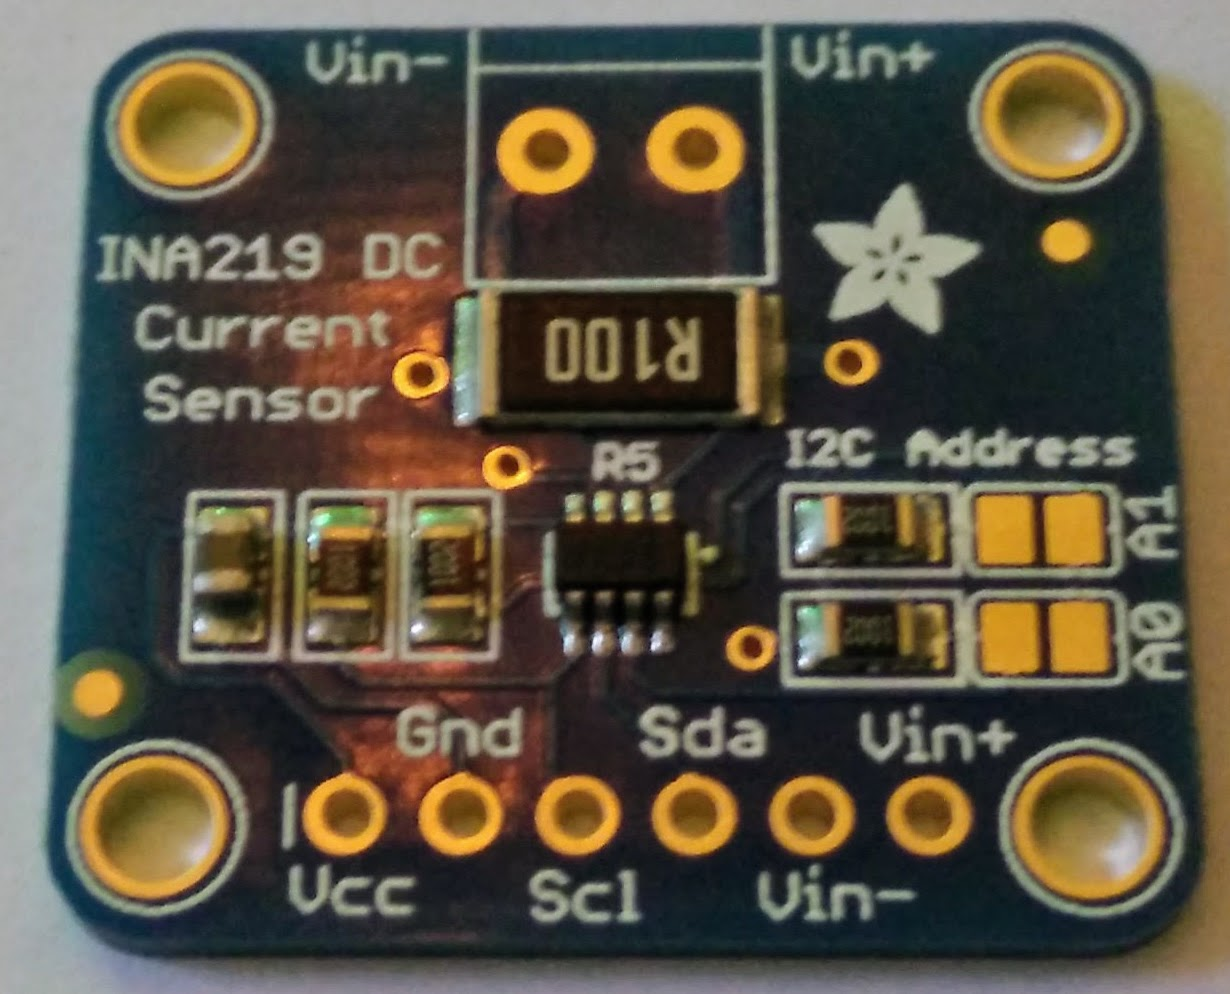
\includegraphics[width=0.5\textwidth]{images/ina219.jpg}
  \caption{INA219, die mit R100 beschriftete Komponente über dem INA219 ist der Messwiderstand.}
  \label{fig:ina219}
\end{figure}

\section{Ergebnisse}
Nachfolgend sind die Ergebnisse für die in dieser Arbeit entstandenen Implementierungen unter den simulierten Bedingungen gelistet.
Es wurde für jedes Konzept jeweils die Implementierung gewählt, die bei den vorherigen Tests innerhalb des Konzepts am besten abgeschnitten hat.\\

%%%%%%%%%%%%%%%%%%%%%%%%%%%%%%%%%%%%%%%%%%%%%%%%%%%%%%%%%%%%%%%%%%
\subsection{WiFi-LLS}
\label{ch:realworld:sec:wifills}
Abbildung \ref{fig:wifills} zeigt den Lastverlauf nach Anschalten der mobilen Einheit für die Implementierung von WiFi-LLS, wenn ein AP zur Verfügung steht. 

\begin{figure}[h!]
  \centering
	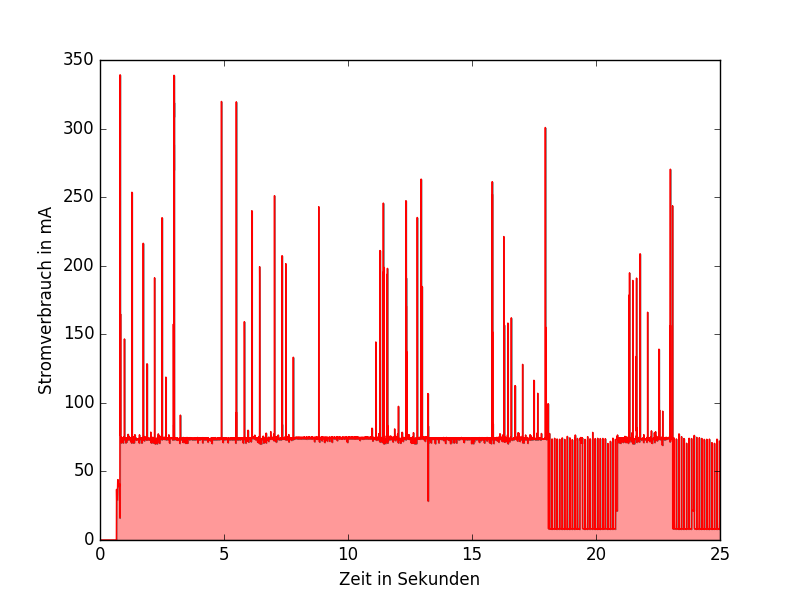
\includegraphics[width=\textwidth]{plots/wifills.png}
  \caption{Lastkurve einer Implementierung von WiFi-LLS.}
  \label{fig:wifills}
\end{figure}

Diese beginnt bei circa einer Sekunde mit dem Scan, nachdem sie diesen beendet hat beginnt sie bei 5 Sekunden mit dem Join Vorgang.\\
Der ESP8266 empfängt während des Join die gesamte Zeit und verbraucht dabei circa 70 Milliamper, nachdem dieser jedoch abgeschlossen ist synchronisiert er sich mit dem AP und lauscht alle 100ms auf den Beacon des AP.
Ist im Beacon eine Aufforderung zum Empfangen für den ESP8266 enhalten empfängt er länger um die Nachricht zu erhalten, ein solches Verhalten ist bei circa 19 Sekunden zu erkennen.\\
Bei 12, 17 und 22 Sekunden werden weitere Scans ausgeführt, diese stehen im Zentrum der Implementierung, da sie implizit die Position bestimmen.
Die rote Kurve in Abbildung \ref{fig:wifillssendv} zeigt diesen Vorgang genauer, ein Scan besteht für jeden gescannten Kanal aus dem Versenden eines Probe Request und anschließenden Empfangen der Probe Responses. 
Abschließend wird ein Paket an den Ortungsserver versendet und der Chip wechselt wieder in einen Zustand, in dem er periodisch die Beacons des AP empfängt.\\

\begin{figure}[h!]
  \centering
	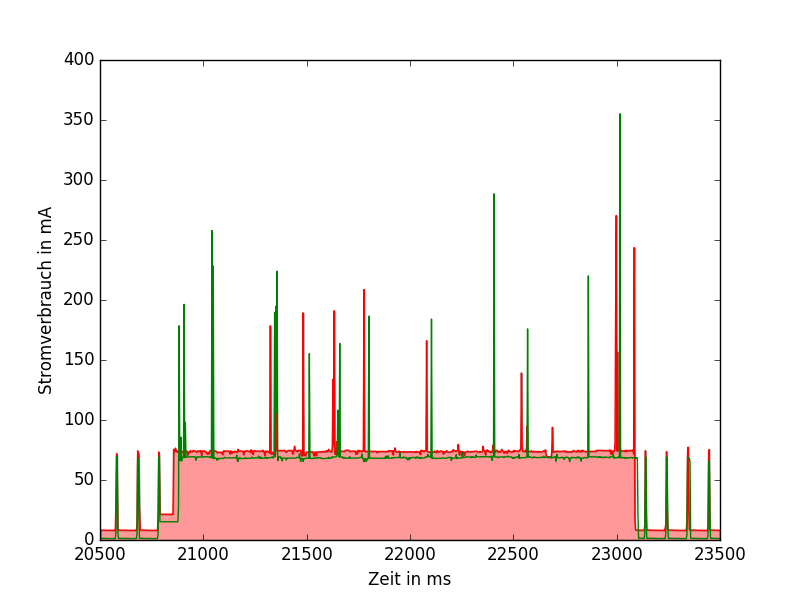
\includegraphics[width=\textwidth]{plots/wifillssendv.png}
  \caption{Lastkurve eines Ortungsvorgangs mit WiFi-LLS.}
  \label{fig:wifillssendv}
\end{figure}

Auffällig ist, dass der Chip circa 8,2 Milliamper verbraucht wenn er nicht empfängt, dagegen gibt das Datenblatt des ESP8266 nur einen Verbrauch von 0,9 Milliamper an.
Das Experiment wurde deshalb mit einem ESP-12F Modul wiederholt, welches nicht auf einem ESP8266 Feather verbaut war, dabei zeigte sich, dass dieses in der selben Situation nur 1,2 Milliamper verbraucht.
Die Lastkurve des einzelnen ESP-12F Modul ist in Abbildung \ref{fig:wifillssendv} grün dargestellt.
Daraus lässt sich schließen, dass die zusätzlichen Komponenten auf dem ESP8266 Feather 7 Milliamper Vebrauch erzeugen, dies ist im Zuge der Laufzeitoptimierung nicht tragbar.\\
Zusätzlich wurde die Implementierung von WiFi-LLS mit nur einem gescannten Kanal geprüft.
Abbildung \ref{fig:wifills1chsend} zeigt den verkürzten Ortungsvorgang.
Da nur ein Kanal gescannt wird, wird nur ein Probe Request versendet.
Nach Empfangen der Antworten wird ein Paket an den Ortungsserver gesendet und der ESP8266 wechselt wieder in den Zustand des periodischen Empfangens.\\

\begin{figure}[h!]
  \centering
	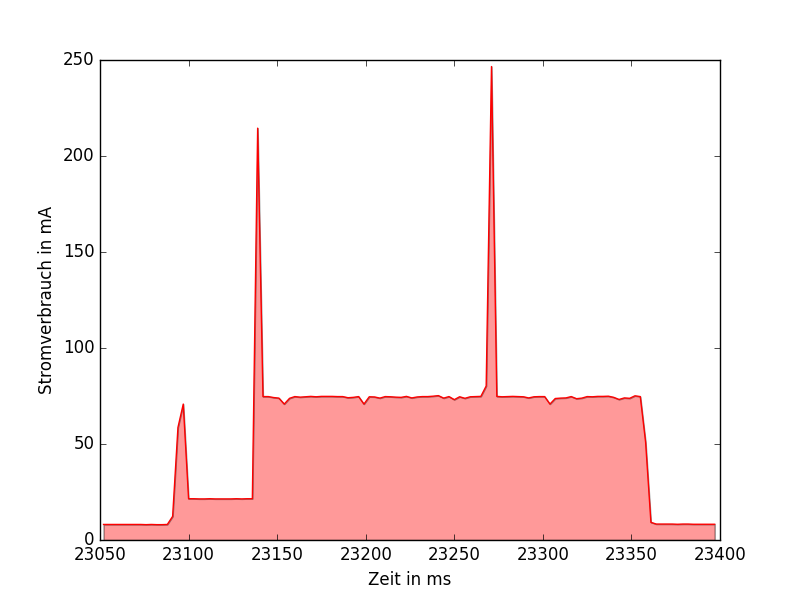
\includegraphics[width=\textwidth]{plots/wifills1chsend.png}
  \caption{Lastkurve des Ortungsvorgangs mit einem gescannten Kanal.}
  \label{fig:wifills1chsend}
\end{figure}

Tabelle \ref{table:wifillsina} listet den durchschnittlichen Verbrauch der Einheiten über eine Stunde.
Die Stromversorgung der Einheiten wurden circa eine Sekunde nach Beginn des Experiments angeschaltet, anschließend treten keine Veränderungen mehr auf.

\begin{table}[h!]
	\centering
	\caption{Energieverbrauch mobiler Einheiten mit WiFi-LLS Implementierung}
	\label{table:wifillsina}
	\begin{tabular}{p{3.5cm}|p{7.5cm}|p{2.5cm}}
		Hardware & Programm & $\varnothing$ Verbrauch in mA \\
		\hline
		ESP8266 Feather & WiFi-LLS alle Kanäle & 42,2 \\
		ESP-12F & WiFi-LLS alle Kanäle & 36,5 \\
		ESP8266 Feather & WiFi-LLS ein Kanal & 18,7 \\
		ESP-12F & WiFi-LLS ein Kanal & 11,4 \\
	\end{tabular}
\end{table}


\subsection{Indirekte Bereichsortung}
\label{ch:realworld:sec:indirekt}
Abbildung \ref{fig:tcphold} zeigt den Lastverlauf nach Anschalten der mobilen Einheit für die Implementierung für Bereichsortung mit aufrecht erhaltener TCP-Verbindung, wenn ein AP zur Verfügung steht. 
Der Beginn des Lastverlaufs ist dem der WiFi-LLS Implementierung ähnlich, es werden ebenfalls Scan und Join durchgeführt.
Da jedoch nur für das Event einer vollständigen (Re-)Assoziation gesendet wird bleibt der ESP8266 anschließend im Zustand des periodischen Empfangens vor Beacons.
Diese wird nur von den Keep Alive Paketen unterbrochen, welche alle 30 Minuten versendet werden.\\

\begin{figure}[h!]
  \centering
	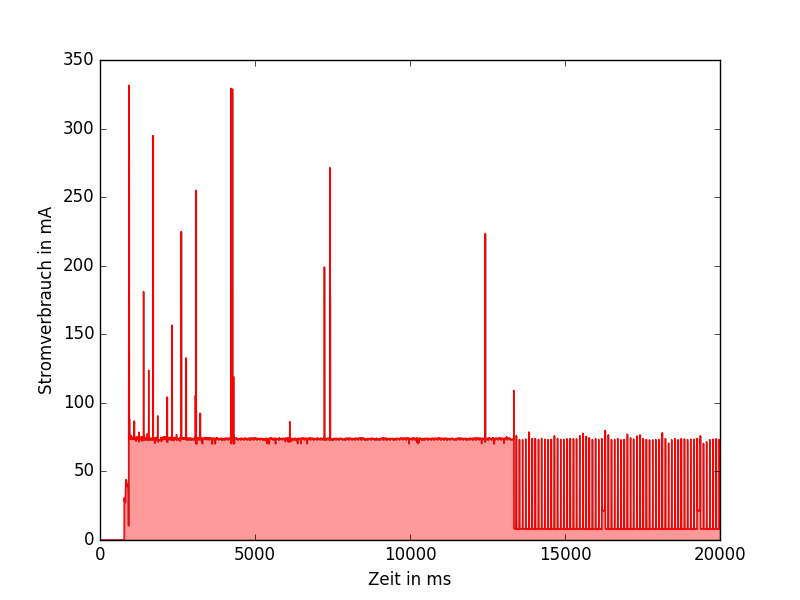
\includegraphics[width=\textwidth]{plots/tcphold.png}
  \caption{Lastkurve einer Implementierung indirekter Bereichsortung, welche eine TCP Verbindung offen hält.}
  \label{fig:tcphold}
\end{figure}

Für die Implementierung mit anschließendem Abbau der TCP-Verbindung kommen zusätzliche Pakete direkt nach dem versenden der Assoziationsinformation an den Ortungsserver hinzu, dafür entfallen die Keep Alive Pakete.
Abbildung \ref{fig:tcpdisco} zeigt dieses Verhalten.\\

\begin{figure}[h!]
  \centering
	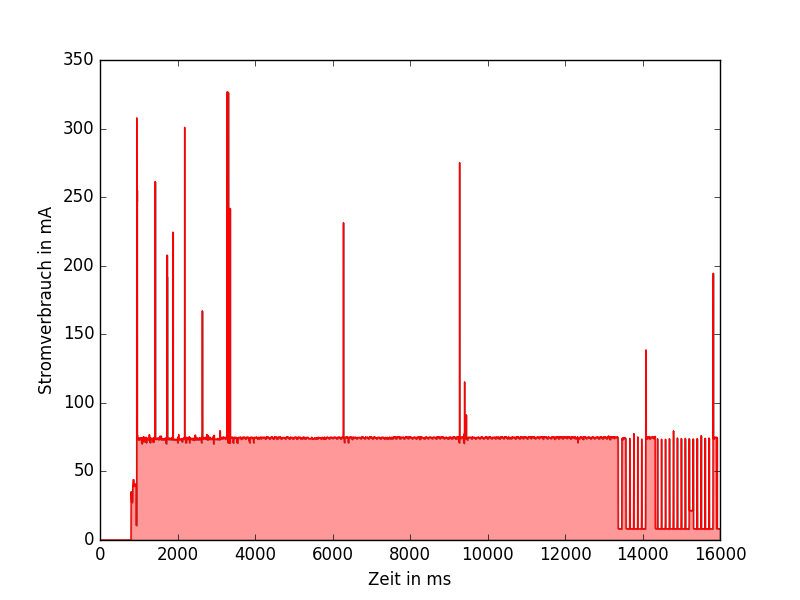
\includegraphics[width=\textwidth]{plots/tcpdisco.png}
  \caption{Lastkurve einer Implementierung indirekter Bereichsortung, welche eine TCP Verbindung nach dem Senden abbaut.}
  \label{fig:tcpdisco}
\end{figure}

Auch diese Implementierungen wurden sowohl mit einem ESP8266 Feather, als auch m,it einem einzelnen ESP-12F Modul getestet, die Ergebnisse sind in Tabelle \ref{table:associatonina} zu finden.

\begin{table}[h!]
	\centering
	\caption{Energieverbrauch mobiler Einheiten mit Bereichsortung}
	\label{table:associatonina}
	\begin{tabular}{p{3.5cm}|p{7.5cm}|p{2.5cm}}
		Hardware & Programm & $\varnothing$ Verbrauch in mA \\
		\hline
		ESP8266 Feather & Bereichsortung TCP Verbindung halten & 15,5 \\
		ESP-12F & Bereichsortung TCP Verbindung halten & 8,8 \\
		ESP8266 Feather & Bereichsortung TCP Verb. schließen & 15,4 \\
		ESP-12F & Bereichsortung TCP Verb. schließen & 8,8 \\
	\end{tabular}
\end{table}

\subsection{RADAR}
Abbildung \ref{fig:radar5s} zeigt den Lastverlauf nach Anschalten der mobilen Einheit für die Implementierung von RADAR, wenn ein AP zur Verfügung steht. 
Der Beginn des Lastverlaufs ist dem der WiFi-LLS Implementierung ähnlich, es werden ebenfalls Scan und Join durchgeführt.\\

\begin{figure}[h!]
  \centering
	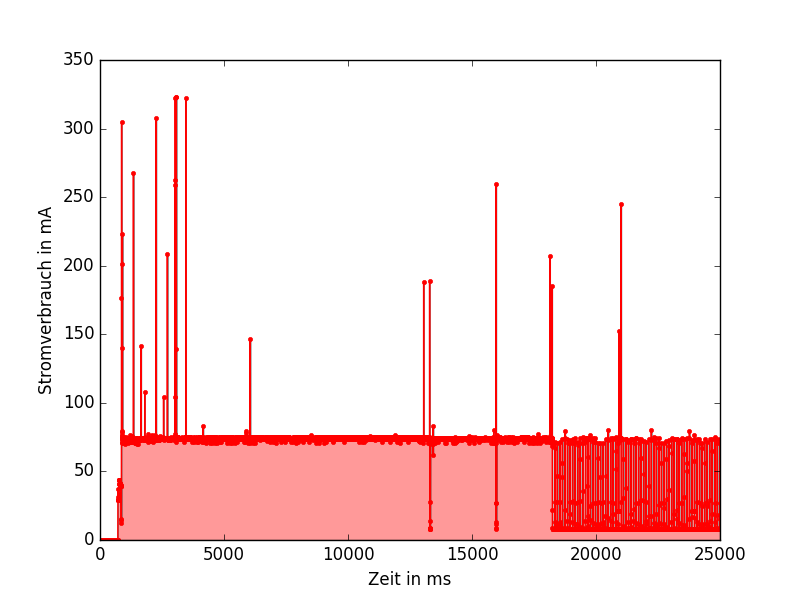
\includegraphics[width=\textwidth]{plots/radar5s.png}
  \caption{Lastkurve einer Implementierung von RADAR.}
  \label{fig:radar5s}
\end{figure}

Abbildung \ref{fig:radar5ssend} zeigt den Sendevorgang der RADAR Implementierung.
Auffällig ist, dass längerfristig empfangen wird, obwohl dies für den Versand des UDP Pakets nicht notwendig ist.\\

\begin{figure}[h!]
  \centering
	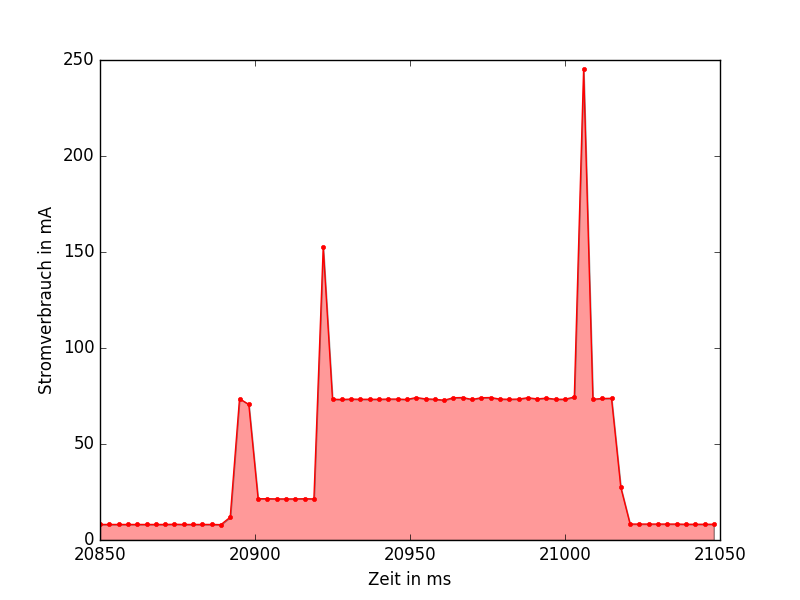
\includegraphics[width=\textwidth]{plots/radar5ssend.png}
  \caption{Lastkurve eines Ortungsvorgangs mit RADAR.}
  \label{fig:radar5ssend}
\end{figure}

In Tabelle \ref{table:radarina} ist der durchschnittliche Verbrauch der RADAR Implementierung über eine Stunde gelistet.
Es wurde sowohl mit dem ESP8266 Feather, als auch mit dem einzelnen ESP-12F gemessen, die mobile Einheit wurde jeweils erst circa eine Sekunde nach Beginn mit Strom versorgt.

\begin{table}[h!]
	\centering
	\caption{Energieverbrauch mobiler Einheiten mit RADAR Implementierung}
	\label{table:radarina}
	\begin{tabular}{p{3.5cm}|p{7.5cm}|p{2.5cm}}
		Hardware & Programm & $\varnothing$ Verbrauch in mA \\
		\hline
		ESP8266 Feather & RADAR & 16,7 \\
		ESP-12F & RADAR & 10,1 \\
	\end{tabular}
\end{table}

\subsection{Probe Request Lokalisierung}
Abbildung \ref{fig:probereqv} zeigt den Lastverlauf für einen Sendevorgang der Probe Request Implementierung, der Verlauf für den ESP8266 Feather ist in Rot und der Verlauf für das ESP-12F Modul ist in Grün dargestellt.\\
Nachdem der ESP8266 aus dem \texttt{deep\_sleep} erwacht beginnt eine circa 100ms andauerne Startphase, danach sendet er die drei Probe Requests.
Anschließend soll der ESP8266 wieder in den \texttt{deep\_sleep} versetzt werden, vorher empfängt er jedoch noch 100ms.
Die restliche Zeit befindet sich der ESP8266 im Tiefschlaf. 
Bei dem ESP-12F Modul ist der INA219 nicht in der Lage einen Vebrauch zu messen, er liegt unter 0,1 Milliamper.\\

\begin{figure}[h!]
  \centering
	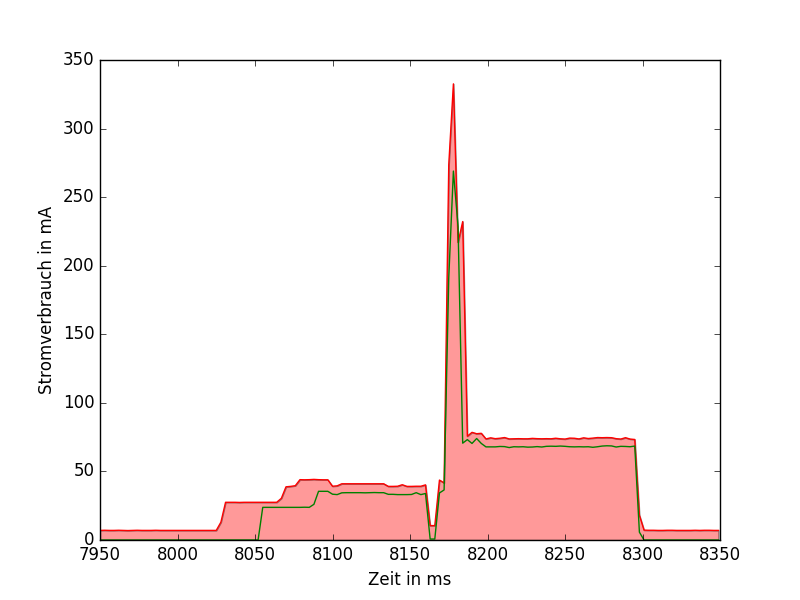
\includegraphics[width=\textwidth]{plots/probereqv.png}
  \caption{Lastkurve eines Ortungsvorgangs mit Probe Requests.}
  \label{fig:probereqv}
\end{figure}

Beim ESP8266 Feather misst er jodoch durchgehend einen Vebrauch von über 7 Milliamper, daraus ergeben sich die Unterschiede in den Messungen, die in Tabelle \ref{probereqina} dargestellt werden.
Es wurde sowohl mit nur einem versendeten Probe Request, als auch mit drei Probe Requests getestet, die Unterschiede im Verbrauch liegen jedoch im Bereich der Messungenauigkeit.

\begin{table}[h!]
	\centering
	\caption{Energieverbrauch mobiler Einheiten mit Probe Request Ortung}
	\label{table:probereqina}
	\begin{tabular}{p{3.5cm}|p{7.5cm}|p{2.5cm}}
		Hardware & Programm & $\varnothing$ Verbrauch in mA \\
		\hline
		ESP8266 Feather & Probe Request drei Kanäle & 9,72 \\
		ESP-12F & Probe Request drei Kanäle & 1,8 \\
		ESP8266 Feather & Probe Request ein Kanal & 9,74 \\
		ESP-12F & Probe Request ein Kanal & 1,82 \\
	\end{tabular}
\end{table}

\subsection{Bluetooth Low Energy Advertising}
\label{ch:realworld:sec:ble}
Abbildung \ref{fig:blue} zeigt den Lastverlauf für den Start einer mobilen Einheit mit Bluetooth Low Energy Advertising.\\
Zu Beginn ist eine Startphase zu erkennen, ab 2 Sekunden nach Start des Experiments ist dann das regelmäßige Muster aus Verbrauch im Ruhezustand und kurzen Verbrauchsspitzen beim Senden zu erkennen.
Die Kürze des Sendevorgangs bedingt die starke Schwankung bei den Lastspitzen, die Samplingrate von 333Hz reicht hier offenbar nicht aus um dem Sendevorgang vollständig zu erfassen.\\

\begin{figure}[h!]
  \centering
	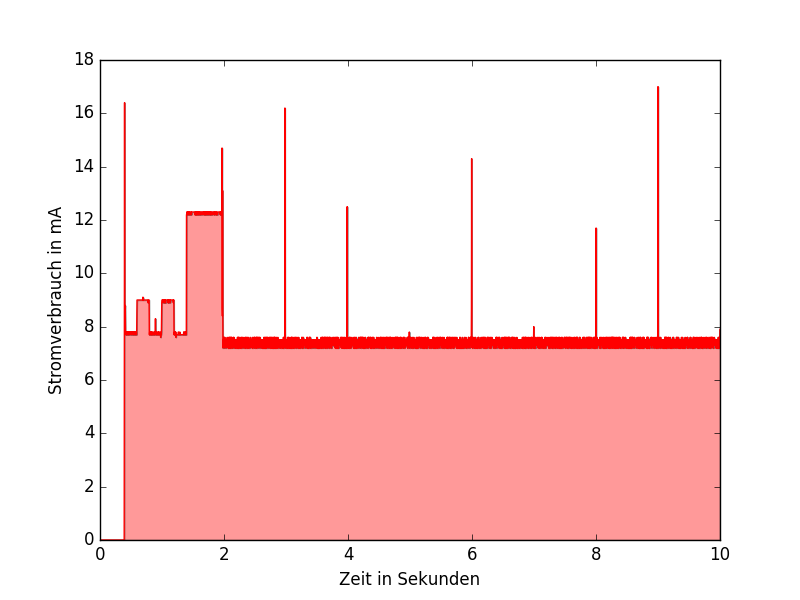
\includegraphics[width=\textwidth]{plots/blue.png}
  \caption{Lastkurve einer Implementierung von Bluetooth Low Energy Advertising.}
  \label{fig:blue}
\end{figure}

Hauptverbrauch liegt jedoch in den 7,2 bis 7,6 Milliamper im Ruhezustand, leider ist in diesem Fall kein einzelnes Modul vorhanden, es kann nur auf dem nRF52 Feather gemessen werden.
Da jedoch die selben Komponenten wie beim ESP8266 Feather zum Einsatz kommen, kann angenommen werden, dass auch der Ruheverbrauch vergleichbar ist, dieser liegt zwischen 7 und 7,1 Milliamper.
Tabelle \ref{table:blueina} zeigt deshalb neben dem gemessenen Verbrauch einen projezierten Verbrauch, bei dem ein Ruheverbrauch von 7,05 Milliamper subtrahiert wurde.

\begin{table}[h!]
	\centering
	\caption{Energieverbrauch mobiler Einheiten mit Bluetooth Low Energy Advertising}
	\label{table:blueina}
	\begin{tabular}{p{3.5cm}|p{7.5cm}|p{2.5cm}}
		Hardware & Programm & $\varnothing$ Verbrauch in mA \\
		\hline
		nRF52 Feather & Bluetooth Low Energy Advertising & 7,37 \\
		nRF52 (projeziert) & Bluetooth Low Energy Advertising & 0,32 \\
	\end{tabular}
\end{table}

\subsection{Lokaliserung mit LoRa}
Der Stromverbrauch der Implementierung mit LoRa wurde mit 5dBm und 23dBm Sendeleistung überprüft
Abbildung \ref{fig:lora23} zeigt den Lastverlauf für den Start einer mobilen Einheit mit LoRA bei 23dBm.\\
Nach einer circa drei sekündigen Startphase wechselt der LoRa Feather in den regulären Betrieb, er sollte dann immer nach zehn Sekunden Ruhezustand senden.
Dieser jedoch vom Zeitgeber nicht ganz eingehalten, die mobile Einheit befindet sich zwischen den Sendevorgängen circa elf Sekunden im Ruhezustand, dies sollte bei der Implementierung beachtet werden.
Im Ruhezustand liegt der Verbrauch des LoRa Feather bei 2,5 bis 2,7 Milliamper, beim Senden unterscheiden sich die Vebräuche je nach Sendeleistung deutlich.\\

\begin{figure}[h!]
  \centering
	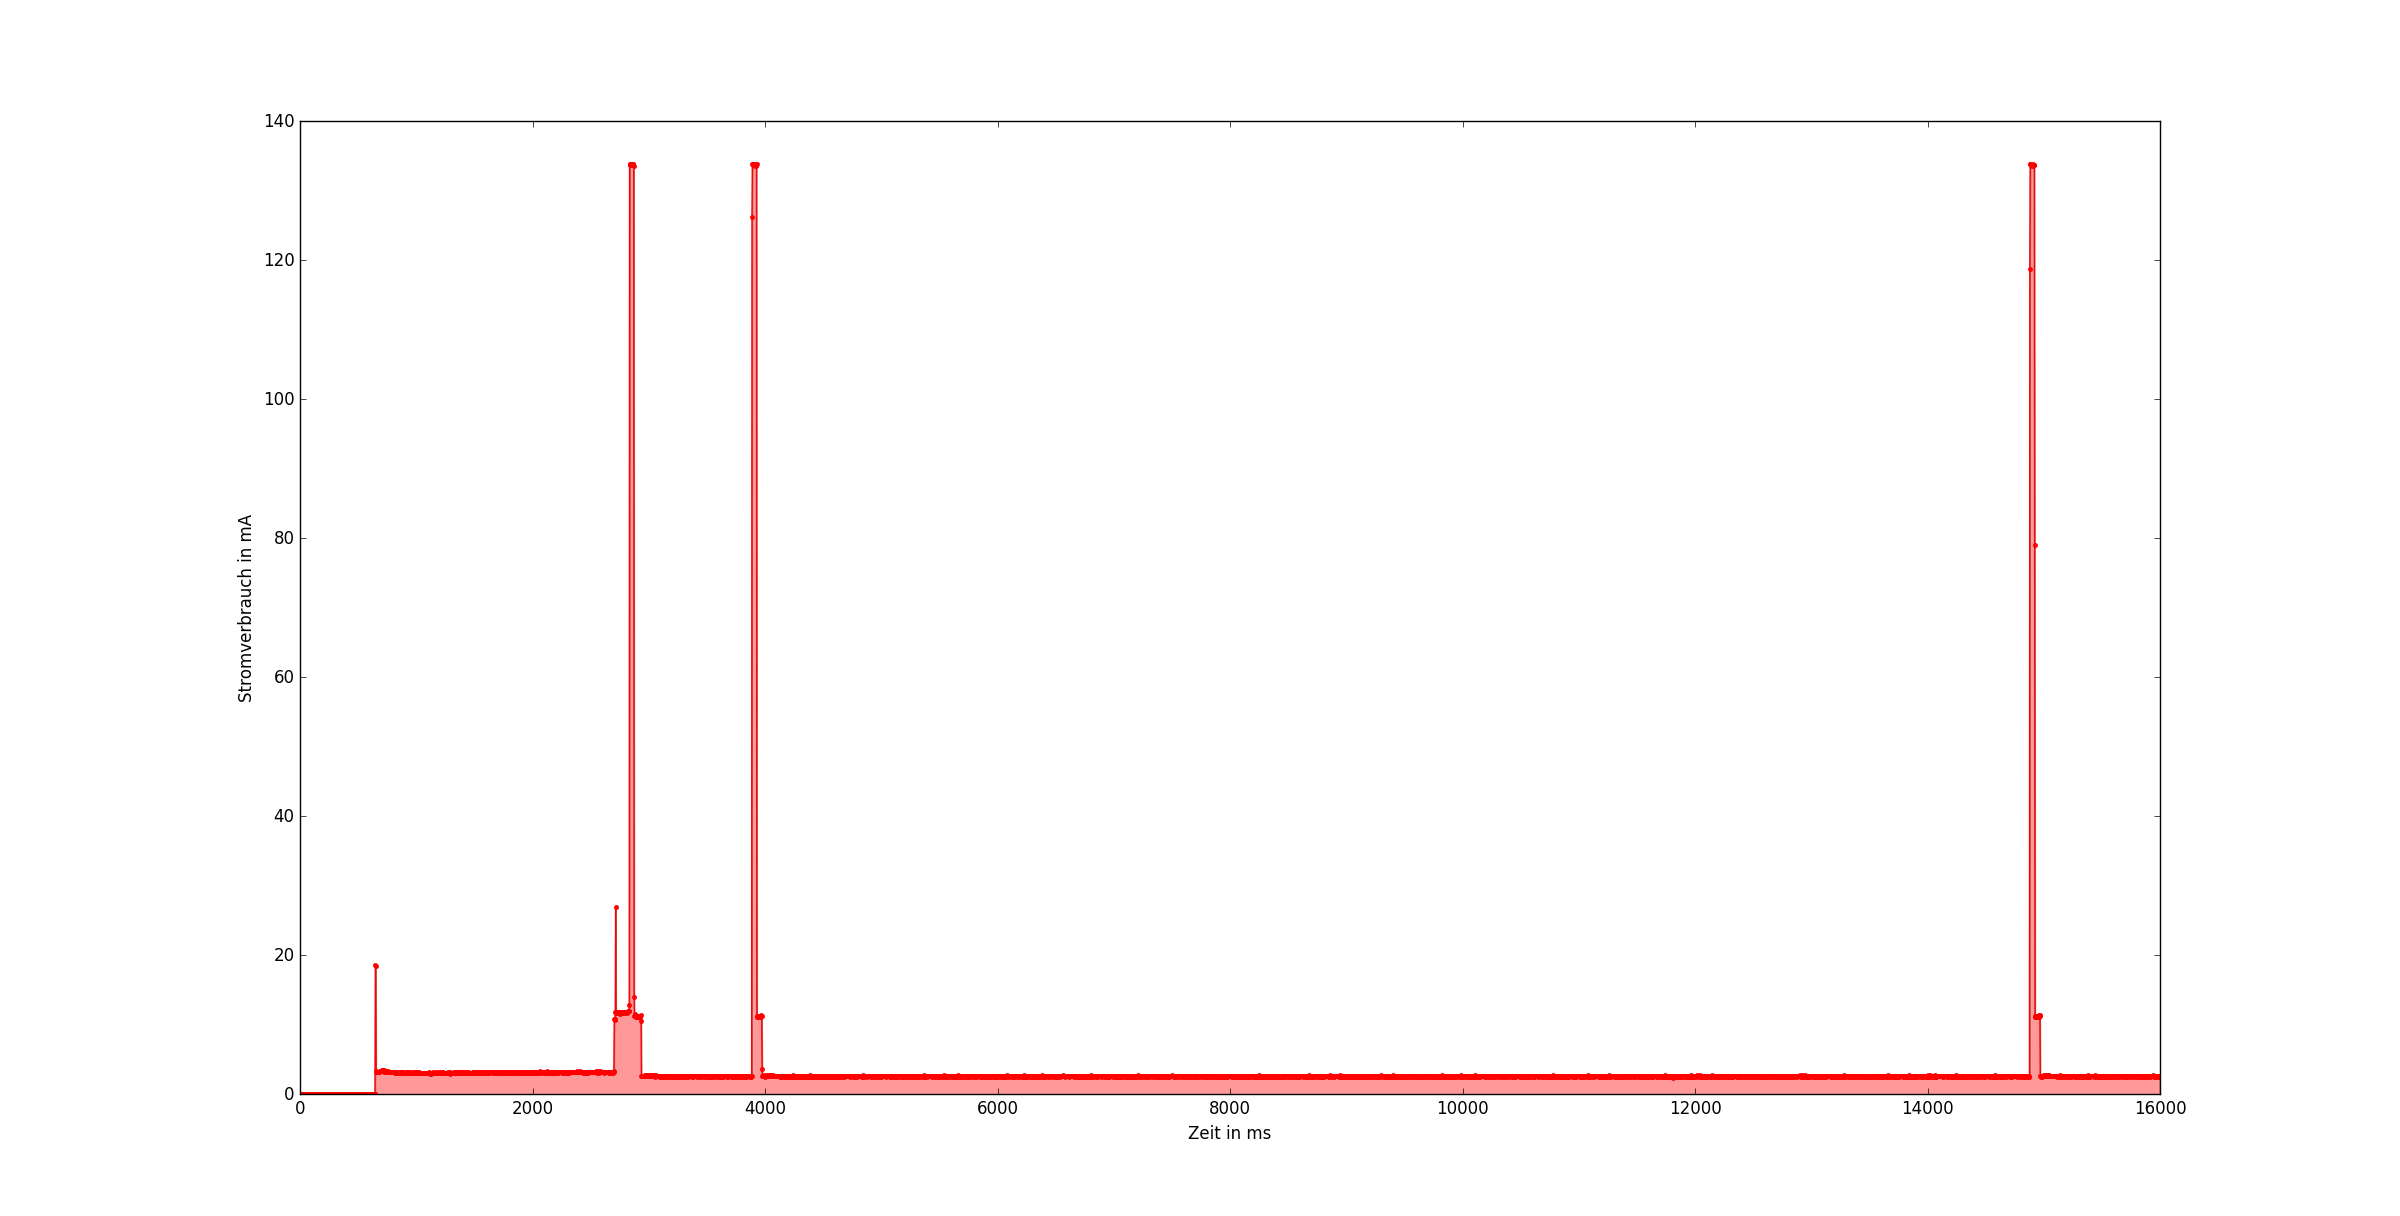
\includegraphics[width=\textwidth]{plots/lora23.png}
  \caption{Lastkurve einer Implementierung mit LoRa.}
  \label{fig:lora23}
\end{figure}

Die Abbildung \ref{fig:lora235send} zeigt die Sendeverbäuche für eine Sendeleistung von 23dBm in Rot und für 5dBm in Grün.
Gut zu erkennen ist hier auch, dass ein Sendevorgang bei LoRa deutlich länger als bei Bluetooth Low Energy dauert, obwohl vergleichbar viele Bits übertragen werden.

\begin{figure}[h!]
  \centering
	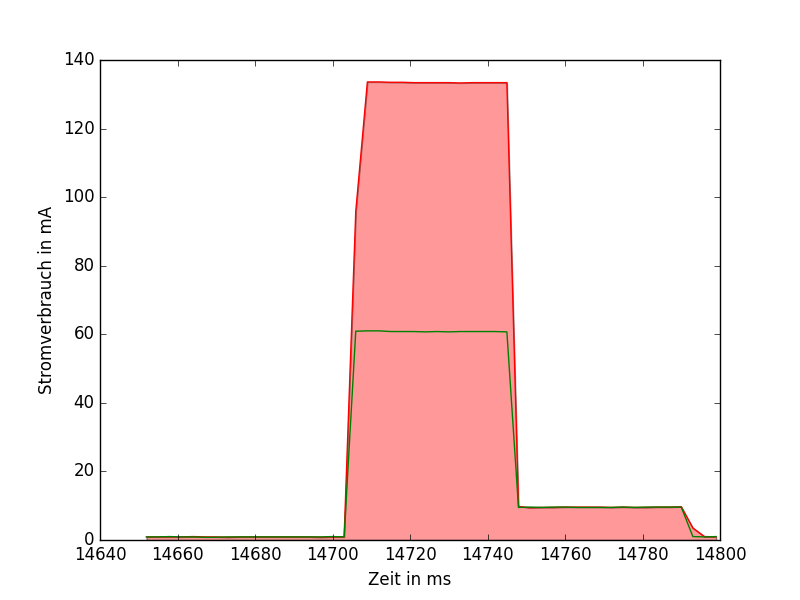
\includegraphics[width=\textwidth]{plots/lora235send.png}
  \caption{Lastkurve eines Ortungsvorgangs mit LoRa.}
  \label{fig:lora235send}
\end{figure}

Die Ergebnisse der Messungen sind in Tabelle \ref{lora235ina} gelistet.\\
Für den LoRa Feather liegt der Ruheverbrauch deutlich niedriger, da jedoch die selben Schaltungen für Akku-Ladung und Spannungsregelung zum Einsatz kommen scheint der CP2104, welcher zum Programmieren des ESP8266 beziehungsweise nRF52 dient, mindestens 4,5 Milliamper zu verbrauchen.

\begin{table}[h!]
	\centering
	\caption{Energieverbrauch mobiler Einheiten mit Bluetooth Low Energy Advertising}
	\label{table:lora235ina}
	\begin{tabular}{p{3.5cm}|p{7.5cm}|p{2.5cm}}
		Hardware & Programm & $\varnothing$ Verbrauch in mA \\
		\hline
		LoRa Feather & LoRa mit 23dBm Sendeleistung & 3,16 \\
		LoRa Feather & LoRa mit 5dBm Sendeleistung & 2,88 \\
	\end{tabular}
\end{table}

%%%%%%%%%%%%%%%%%%%%%%%%%%%%%%%%%%%%%%%%%%%%%%%%%%%%%%%%%%%%%%%%%%%%%%%%

\section{Bewertung}
Die Implementierungen, die dem Netzwerk beitreten verbrauchen deutlich mehr Strom, wenn kein Access Point in Reichweite ist, dem sie beitreten können.
Dies macht sie ungeeignet für ein Szenario mit lückenhafter WLAN Abdeckung.
Die Implementierungen die auf dem Versenden von Probe Requests beziehungsweise BLE Advertising Paketen basieren sind nicht von der Basisstation als Gegenstelle abhänging und verbrauchen deshalb auch in diesem Szeanrio auch nicht mehr Energie.
Die BLE Advertising Implementierung ist dabei bezüglich der Laufzeit trotz des kürzeren Sendeintervalls der Probe Request Implementierung weit überlegen.
